\documentclass[12pt, a4paper]{article}

\usepackage{amsmath}
\usepackage{array}
\usepackage{amsmath}
\usepackage[portuguese]{babel}
\usepackage{chngpage}
\usepackage{float}
\usepackage[a4paper, margin=2cm]{geometry}
\usepackage{graphicx}
\usepackage{hyperref}
\usepackage{listings}
\usepackage{setspace}
\usepackage{xcolor}

\lstdefinestyle{codestyle}{
    commentstyle=\color{teal},
    keywordstyle=\color{blue},
    numberstyle=\ttfamily\color{gray},
    stringstyle=\color{red},
    basicstyle=\ttfamily\footnotesize,
    breakatwhitespace=false,
    breaklines=false,
    keepspaces=true,
    numbers=none,
    showspaces=false,
    showstringspaces=false,
    showtabs=false,
    tabsize=4
}
\lstset{style=codestyle}

\title{\Huge \textbf{Computação Gráfica \\ \Large Trabalho Prático -- Fase II}}
\date{30 de março 2025}
\author{Grupo 3}

\begin{document}

\begin{center}
    
\includegraphics[width=0.25\textwidth]{res/cover/EE-C.eps}
\end{center}

\chardef\_=`_
\onehalfspacing
\setlength{\parskip}{\baselineskip}
\setlength{\parindent}{0pt}
\def\arraystretch{1.5}

{\let\newpage\relax\maketitle}
\maketitle
\thispagestyle{empty}

\vspace*{\fill}

\begin{adjustwidth}{-2cm}{-2cm} % These values only need to be large enough to center the table
    \begin{center}
        \begin{tabular}{>{\centering}p{0.25\textwidth}
                        >{\centering}p{0.25\textwidth}
                        >{\centering}p{0.25\textwidth}
                        >{\centering\arraybackslash}p{0.25\textwidth}}
            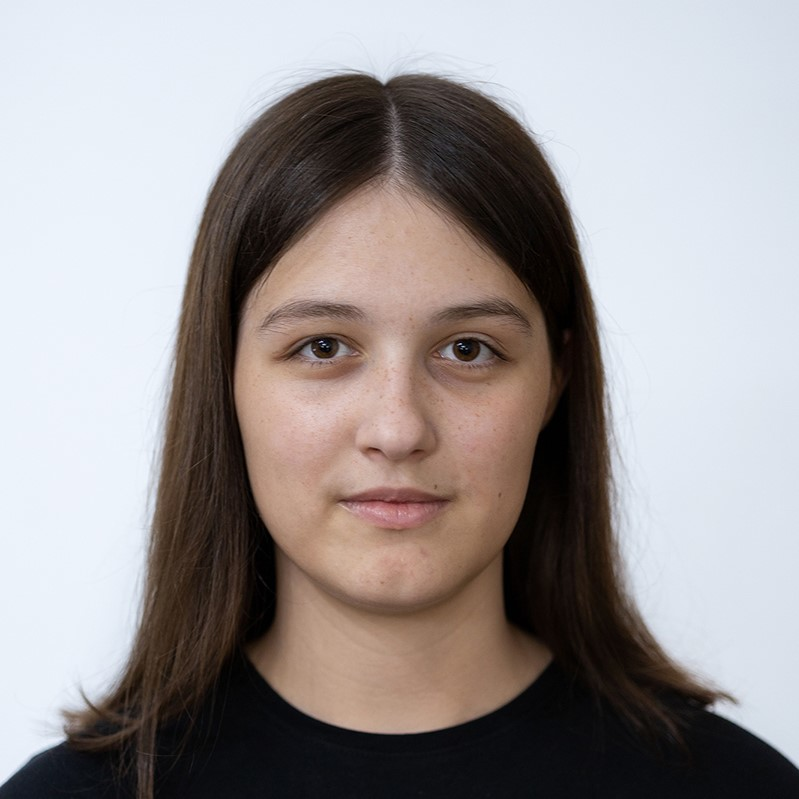
\includegraphics[width=3.5cm]{res/cover/A104437.png} &
            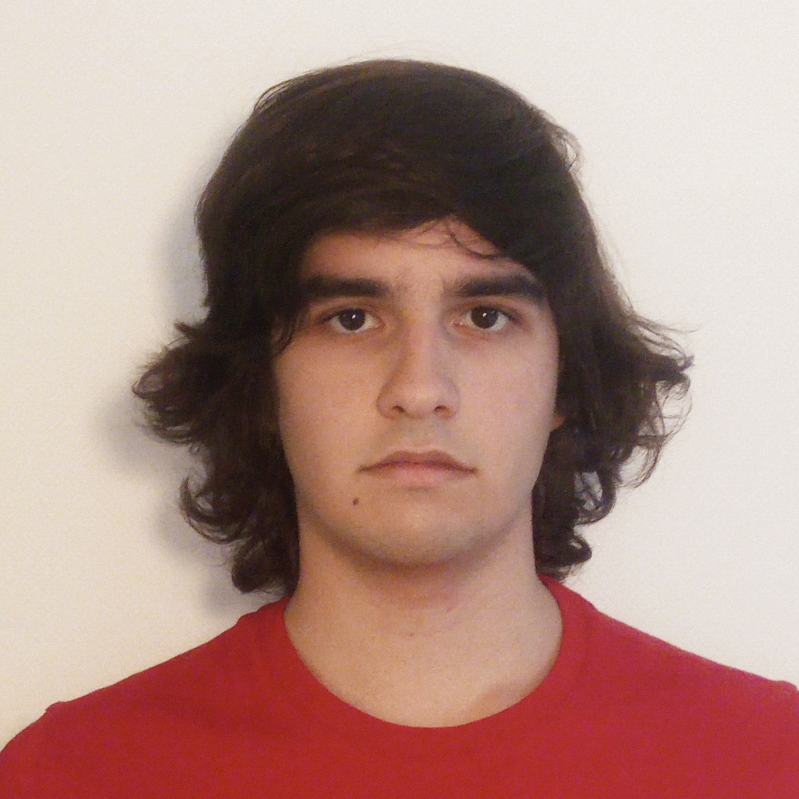
\includegraphics[width=3.5cm]{res/cover/A104348.png} &
            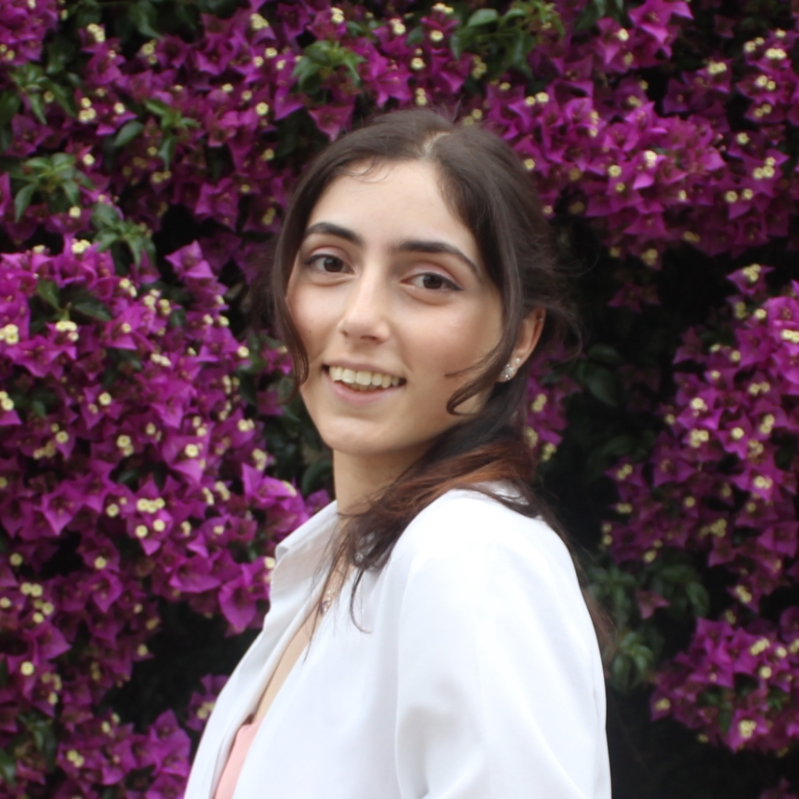
\includegraphics[width=3.5cm]{res/cover/A90817.png} &
            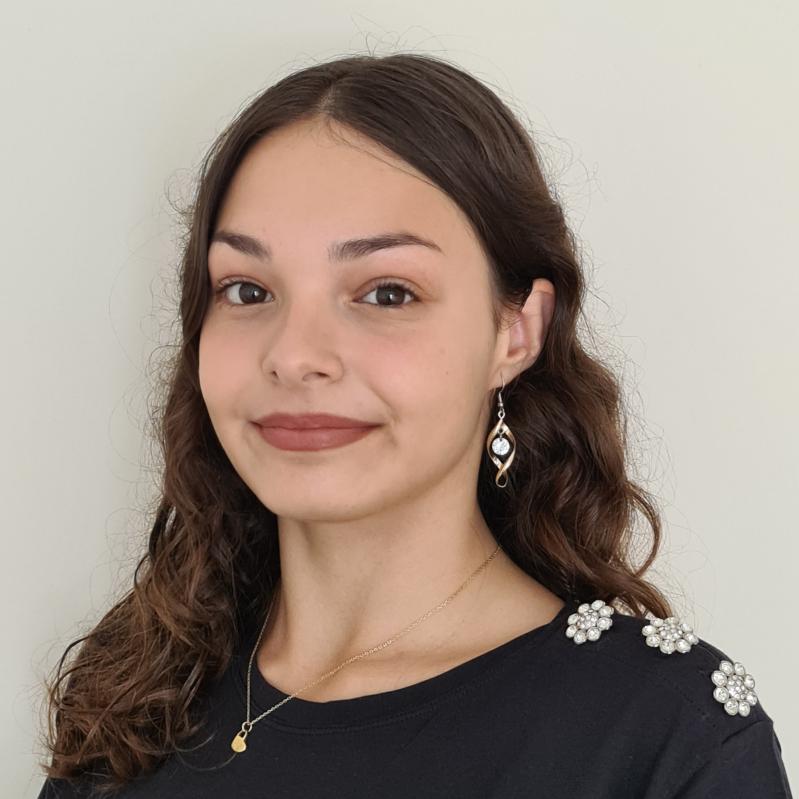
\includegraphics[width=3.5cm]{res/cover/A104179.png} \\

            Ana Oliveira & Humberto Gomes & Mariana Cristino & Sara Lopes \\
            A104437      & A104348        & A90817           & A104179
        \end{tabular}
    \end{center}
\end{adjustwidth}

\pagebreak

\begin{abstract}
    \textbf{\color{red} TODO - resumo}
\end{abstract}

\section{Transformações}

\textbf{\color{red} TODO - transformações}

\section{Modelo estático do sistema solar}

\textbf{\color{red} TODO - sistema solar}

\section{Extras}

\textbf{\color{red} TODO - extras}

\section{Resultados obtidos}

Nesta fase, implementámos câmaras orbital e livre, transformações hierárquicas, frustum culling e
novas primitivas geométricas. Os resultados incluem novos modelos de primitivas gerados pelo
\texttt{generator}, testes de renderização, uma representação funcional do sistema solar e a
implementação de \textit{frustum culling}.

\subsection{Figuras geométricas geradas}

Os seguintes modelos foram criados utilizando o \texttt{generator} implementado:

\begin{figure}[H]
    \centering
    \begin{minipage}{0.48\textwidth}
        \centering
        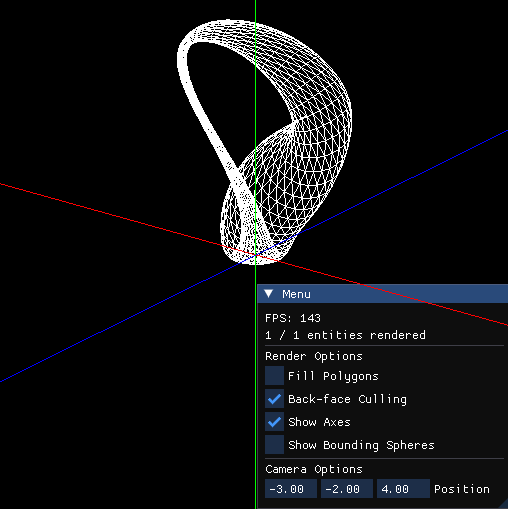
\includegraphics[width=0.5\textwidth]{res/phase2/results/KleinBottle.png}
        \caption{Garrafa de Klein (\texttt{kleinBottle})}
    \end{minipage}\hfill
    \begin{minipage}{0.48\textwidth}
        \centering
        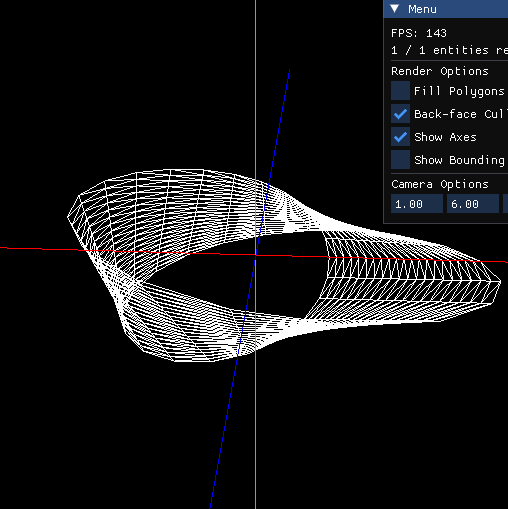
\includegraphics[width=0.5\textwidth]{res/phase2/results/MobiusStrip.png}
        \caption{Fita de Möbius (\texttt{möbius strip})}
    \end{minipage}
\end{figure}

\begin{figure}[H]
    \centering
    \begin{minipage}{0.48\textwidth}
        \centering
        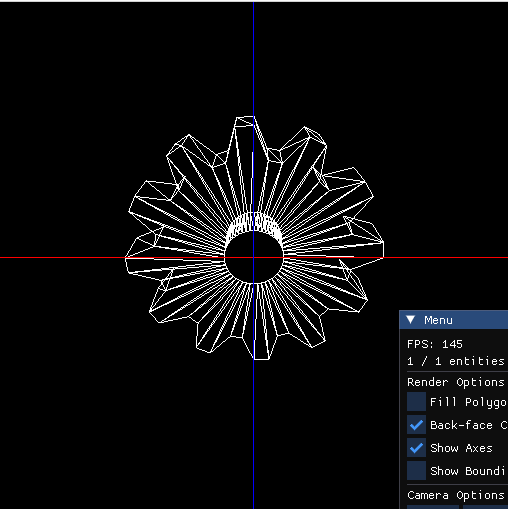
\includegraphics[width=0.5\textwidth]{res/phase2/results/Gear.png}
        \caption{Roda dentada (\texttt{gear})}
    \end{minipage}\hfill
\end{figure}

\subsection{Cenas fornecidas pela docência da UC}

A docência da UC forneceu, juntamente com o enunciado do trabalho, algumas cenas a serem testadas no
trabalho. A \texttt{engine} renderizou-as como esperado:

\begin{figure}[H]
    \begin{adjustwidth}{-2cm}{-2cm}
        \centering
        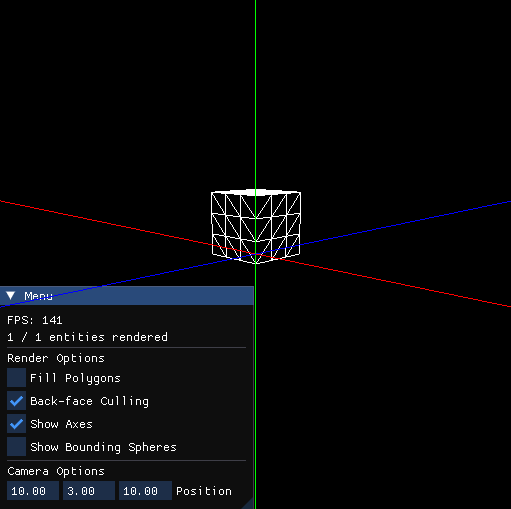
\includegraphics[width=0.26\textwidth]{res/phase2/results/Test1.png}
        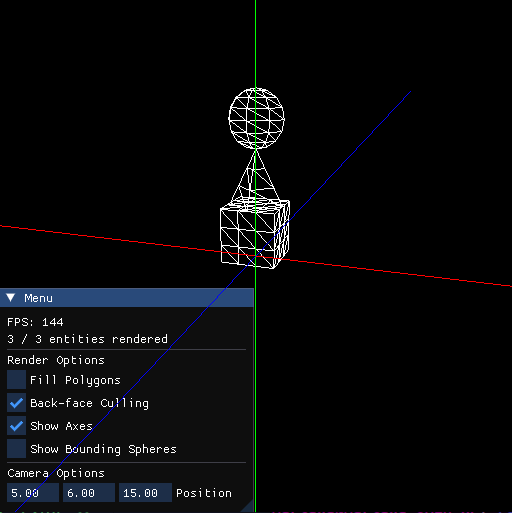
\includegraphics[width=0.26\textwidth]{res/phase2/results/Test2.png}
        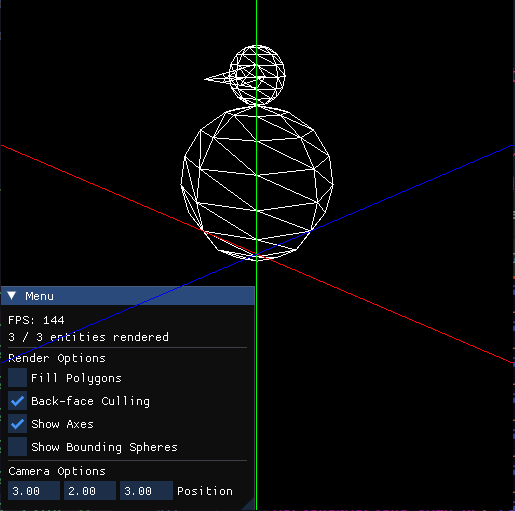
\includegraphics[width=0.26\textwidth]{res/phase2/results/Test3.png}
        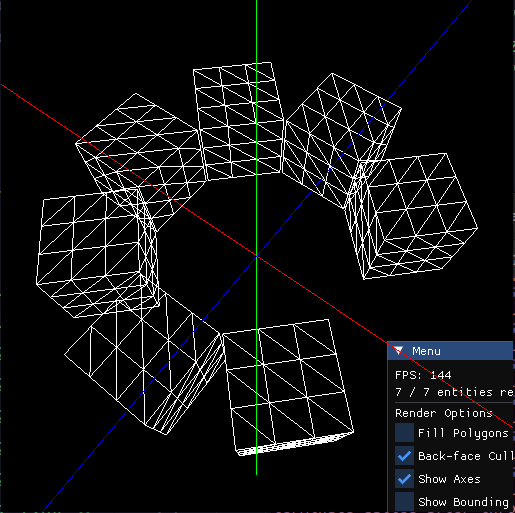
\includegraphics[width=0.26\textwidth]{res/phase2/results/Test4.png}
        \caption{Renderização das cenas de teste fornecidas pela docência da UC.}
    \end{adjustwidth}
\end{figure}

\subsection{Sistema Solar}

A hierarquia implementada produziu com sucesso as órbitas e relações de escala do sistema solar.

\begin{figure}[H]
    \centering
    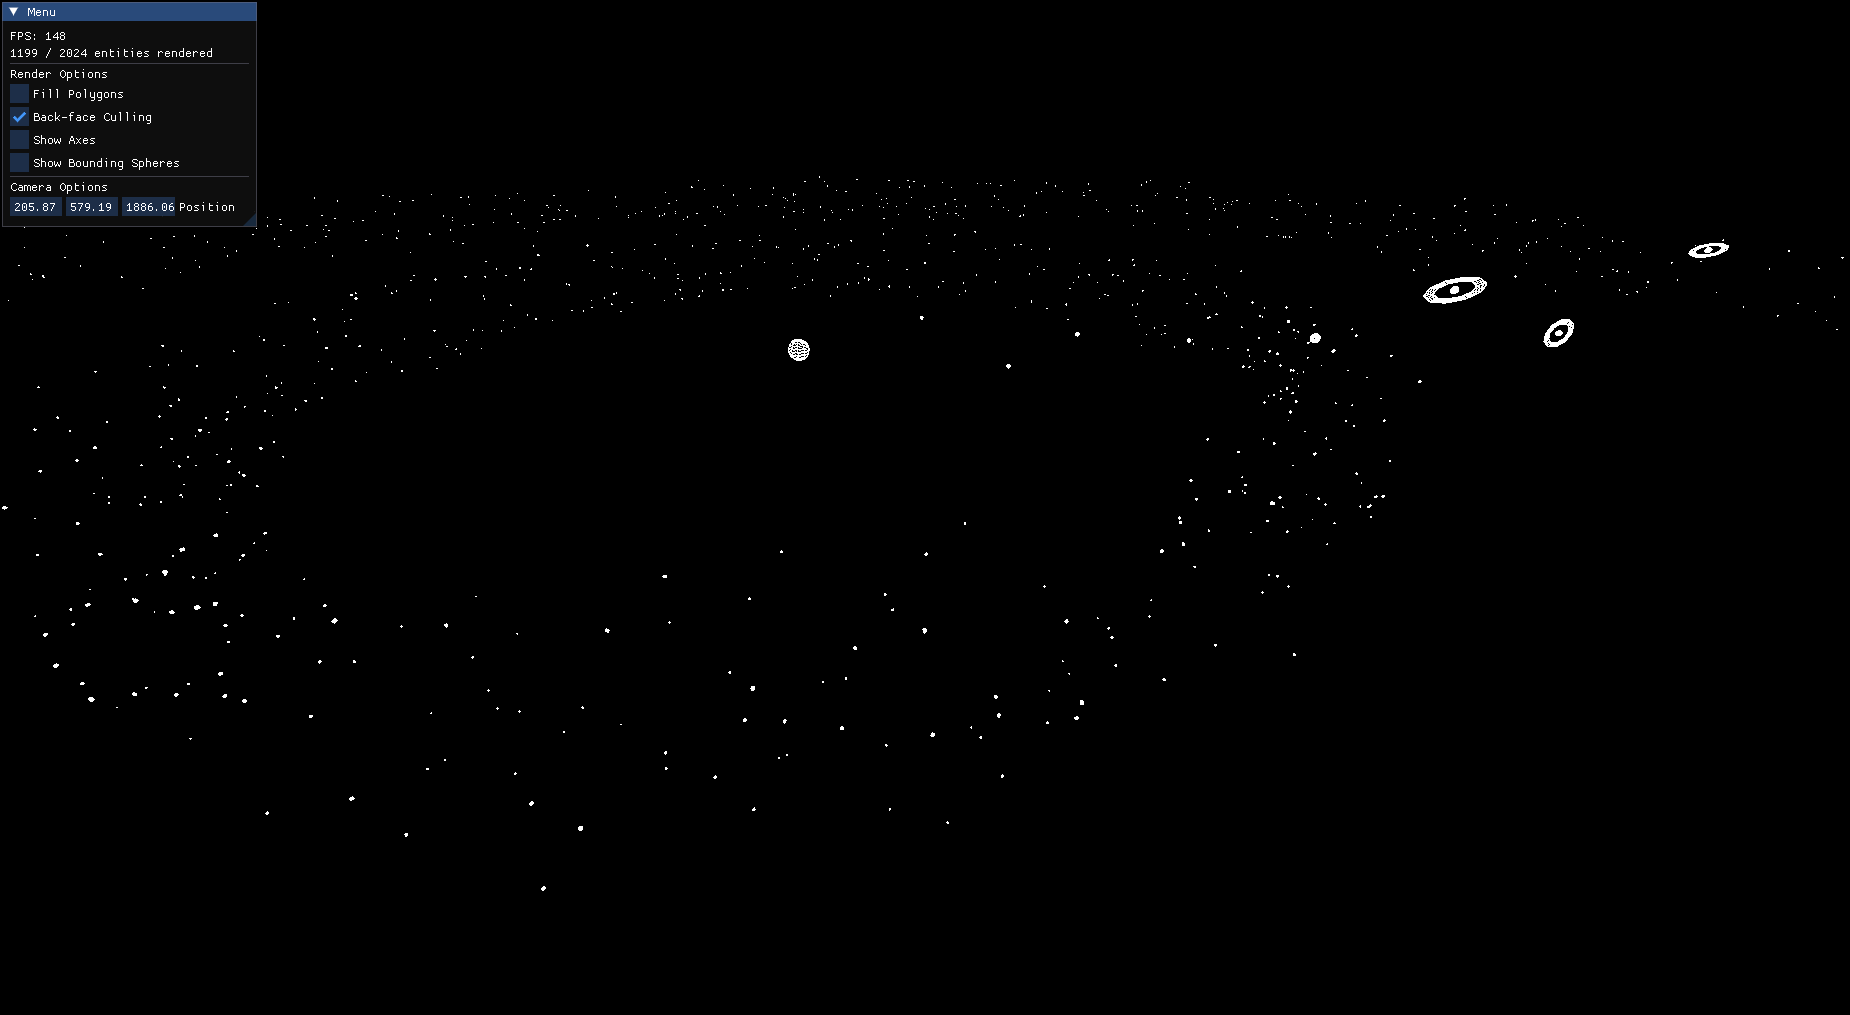
\includegraphics[width=0.5\textwidth]{res/phase2/results/SolarSystem.png}
    \caption{Renderização do sistema solar.}
\end{figure}

\subsection{Frustum Culling}

O \textit{frustum culling} utiliza as esferas vermelhas para verificar se um objeto
se encontra dentro do campo de visão da câmara. Se a esfera estiver dentro da área visível, o
modelo correspondente é renderizado. Os objetos que se encontrem fora do \textit{frustum} têm as
suas esferas ignoradas, o que evita um processamento desnecessário.

\begin{figure}[H]
    \begin{adjustwidth}{-2cm}{-2cm}
        \centering
        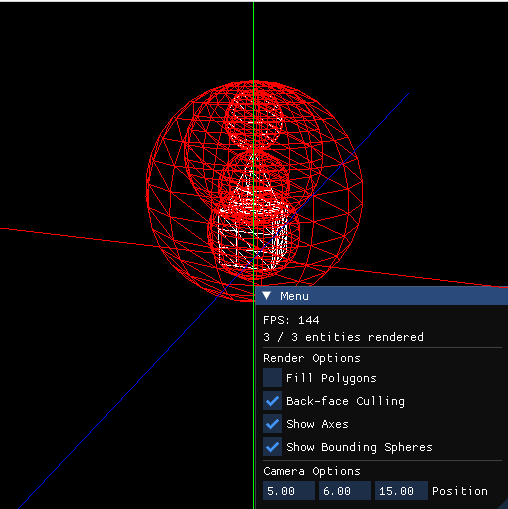
\includegraphics[width=0.4\textwidth]{res/phase2/results/FrustumCulling.png}
        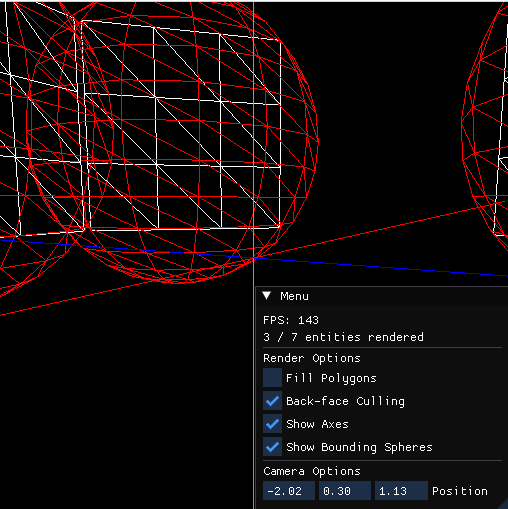
\includegraphics[width=0.4\textwidth]{res/phase2/results/FrustumCullingpt2.png}
        \caption{Frustum Culling}
    \end{adjustwidth}
\end{figure}

\section{Conclusão e Trabalho Futuro}

\textbf{\color{red} TODO - conclusão}

\begingroup
\section{Bibliografia}
\renewcommand{\section}[2]{}

\begin{thebibliography}{9}
    \bibitem{exemplo}
        \href{https://youtu.be/dQw4w9WgXcQ}{Um item de exemplo na bibliografia}
\end{thebibliography}
\endgroup

\end{document}
